\pdfminorversion=7
\pdfsuppresswarningpagegroup=1
\documentclass[11pt]{article}

\usepackage[margin=1in]{geometry}
\usepackage{amsmath,amssymb}
\usepackage{amsthm}
\usepackage{array}
\usepackage{authblk}
\usepackage{booktabs}
\usepackage{float}
\usepackage{graphicx}
\usepackage{longtable}
\usepackage{tikz}
\usepackage{hyperref}
\usepackage{xcolor}
\usetikzlibrary{arrows.meta,positioning,calc,fit}

\hypersetup{
    colorlinks=true,
    linkcolor=blue,
    citecolor=blue,
    urlcolor=blue,
    pdftitle={A Decomposition-Aware Multi-Scale Mamba Model for Nonstationary Financial Forecasting},
    pdfauthor={Bing Mo, Wei Zhang, Xianzhong Zhou, Qi Zheng, Feng Yang},
    pdfkeywords={financial forecasting, nonstationary time series, Mamba, state-space models, multi-scale analysis}
}

\newtheorem{proposition}{Proposition}
\newcommand{\runningtitle}{Multi-Scale Mamba Forecasting}
\title{A Decomposition-Aware Multi-Scale Mamba Model for Nonstationary Financial Forecasting}
\author[1]{Bing Mo\thanks{Corresponding author: \href{mailto:hitmbzq@126.com}{hitmbzq@126.com}}}
\author[1]{Wei Zhang}
\author[2]{Xianzhong Zhou\thanks{Corresponding author: \href{mailto:zhouxzh@gdut.edu.cn}{zhouxzh@gdut.edu.cn}}}
\author[3,4]{Qi Zheng\thanks{Corresponding author: \href{mailto:mbzq@163.com}{mbzq@163.com}}}
\author[4]{Feng Yang}
\affil[1]{Frontier Interdisciplinary Domain, Beijing Institute of Technology, Zhuhai, China}
\affil[2]{School of Integrated Circuits, Guangdong University of Technology, Guangzhou, China}
\affil[3]{Tsinghua Shenzhen International Graduate School, Tsinghua University, Shenzhen, China}
\affil[4]{Silictec (Shenzhen) Electronic Technology Co., Ltd., Shenzhen, China}
\date{}

\begin{document}

\maketitle

\begin{center}
\small\textit{Running title: \runningtitle}
\end{center}

\begin{center}
\small\textbf{Internal draft. The theory and data analysis are complete; final out-of-sample model results are pending.}
\end{center}

\begin{abstract}
Financial level series exhibit persistent levels, changing volatility, and evolving cross-series relationships, conditions under which model rankings can depend strongly on the evaluation protocol.
We define a prospectively frozen benchmark of four daily financial panels: foreign exchange, U.S. Treasury yields, cross-asset indicators, and cryptoassets.
Each panel yields a univariate-input task and a multivariate-input, single-target task.
Nine learned models---five non-Mamba baselines, S-Mamba, and three decomposition or multi-scale Mamba variants---are compared with last-value, random-walk-with-drift, ARIMA, and, for multivariate tasks, VAR-on-differences references at horizons of 1, 5, 20, 60, 120, and 252 observations.
Hyperparameters are selected using 2021--2022 validation data after training through 2020; the 2023--2026 final period remains inaccessible until the complete selection audit passes.
Selection-safe diagnostics show that all four training targets are consistent with nonstationary levels under the prespecified ADF/KPSS diagnostic pair, while validation-period mean shifts range from 0.51 to 7.75 training standard deviations in magnitude and first-difference volatility ratios range from 0.82 to 4.52.
Final neural estimates will average five seeds, and paired loss contrasts will use a moving-block bootstrap with multiplicity adjustment.
Because the locked evaluation is still running, this interim manuscript reports the protocol and data characterization but makes no performance claim.
\end{abstract}

\section{Introduction}

Long-horizon forecasting requires a model to extract predictive structure while the usefulness of past observations changes with the forecast length.
Modern approaches address this problem through efficient attention, decomposition, temporal patches, inverted tokenization, and multi-scale representations \cite{informer,autoformer,dlinear,patchtst,timesnet,itransformer}.
Their relative performance is strongly protocol- and dataset-dependent: lookback length, normalization, optimization budget, temporal split, and evaluation metric can alter model rankings \cite{m4,m5,tsf-survey}.

Nonstationarity adds a second difficulty.
Changes in level, scale, trend, volatility, or local dynamics can make future windows differ from the observations used for training.
RevIN addresses window-level distribution shift through reversible normalization, while Non-stationary Transformers combine stationarization with a learned mechanism intended to restore useful nonstationary information \cite{revin,nonstationary-transformer}.
Decomposition models provide a complementary inductive bias by separating slowly varying and residual components before forecasting \cite{autoformer,fedformer,dlinear}.

Mamba offers input-selective state-space sequence modeling with linear scaling in sequence length \cite{mamba}.
Forecasting adaptations differ in how they tokenize time and variables, scan in one or two directions, and combine temporal resolutions \cite{smamba,bimamba,mambats,timemachine,tsmamba}.
Recent multi-scale and decomposition-enhanced Mamba studies make this design space increasingly crowded \cite{msmamba,karma,dmamba}.
An efficient or more elaborate sequence operator is therefore not, by itself, evidence of improved forecasting.

The requirement for a strong reference forecast is particularly important for persistent financial level series.
Forecasting competitions repeatedly show that simple methods can remain difficult to beat \cite{m4,m5}, while financial forecasting reviews emphasize sensitivity to target definition, regime changes, and evaluation design \cite{finance-dl-survey}.
A model comparison on price or exchange-rate levels should therefore include a last-observation forecast before attributing an observed difference to architectural sophistication.

This study reports the completed repository benchmark for four Mamba configurations: S-Mamba, a decomposition variant (NS-Mamba-D), a multi-scale decomposition variant (MS-Mamba-MD), and a patch-temporal multi-scale decomposition variant (PMS-Mamba-PD).
They are compared with ten tuned neural baselines and a deterministic last-value forecast on GLD and Exchange under single-target (S-mode) forecasting.
Both datasets use 12 forecast lengths from 1 to 360 observations.
Within each final neural sweep, candidate configurations are selected by validation performance and evaluated on the test period.
However, earlier GLD test results were consulted during architecture development; consequently, the present evaluation is descriptive rather than an untouched confirmatory test.

The contributions are:
\begin{itemize}
    \item a traceable two-series benchmark covering 14 trained models, a deterministic last-value reference, and 12 forecast lengths;
    \item an implementation-grounded comparison of inverted, decomposition, multi-scale, and patch-temporal Mamba configurations against diverse neural alternatives;
    \item a reproducible persistence calculation showing that the strongest learned model differs by series and that last-value is best on Exchange under the current metric; and
    \item an explicit account of test-period reuse, single-seed uncertainty, overlapping forecast windows, search-budget asymmetry, post hoc dataset exclusion, and univariate tokenization.
\end{itemize}

\section{Related Work}

\subsection{Nonstationary Representations for Forecasting}

Forecasting under distribution shift has motivated both reversible normalization and architecture-level responses.
RevIN normalizes each input instance and reverses the transformation at the output \cite{revin}; Non-stationary Transformers add a learned de-stationary mechanism because normalization can also remove predictive information \cite{nonstationary-transformer}.
Decomposition methods separate slow and residual structure so that a single representation need not explain every temporal scale \cite{autoformer,fedformer,dlinear}.
PatchTST, N-BEATS, and N-HiTS provide complementary examples of patching, basis expansion, and explicit multi-rate temporal structure \cite{patchtst,nbeats,nhits}.
PMS-Mamba uses these ideas as representation choices and does not interpret its components as uniquely identified financial processes.

\subsection{Mamba Tokenization for Time Series}

Mamba replaces self-attention with an input-selective state-space recurrence \cite{mamba}.
S-Mamba applies bidirectional Mamba blocks over variable tokens \cite{smamba}; Bi-Mamba+, MambaTS, and TimeMachine study bidirectionality, scan directions, and multiple Mamba pathways \cite{bimamba,mambats,timemachine}.
The distinction between variable tokens and temporal tokens is central in the present work.
Inverted representations can capture cross-variable relations when several variables are available \cite{itransformer}, but they reduce a target-only input to one token.
PMS-Mamba instead makes its selective state-space encoder operate on temporal patch sequences at each scale.

Several recent studies also combine Mamba with multiple scales or decomposition.
ms-Mamba uses several temporal sampling rates \cite{msmamba}; KARMA combines multilevel decomposition with multi-scale Mamba blocks \cite{karma}; and DMamba assigns different modules to decomposed components \cite{dmamba}.
The contribution here is not a priority claim for these individual ideas.
It is a specific patch-based composition, a direct account of why it is needed for univariate Mamba inputs, and an evaluation focused on nonstationary financial levels.

\subsection{Financial Data Analysis and Evaluation}

Financial time-series studies are sensitive to the definition of the target, temporal split, regime coverage, and reference forecast \cite{finance-dl-survey}.
For persistent levels, last-value, drift, and classical univariate or multivariate forecasts are necessary references; forecasting competitions also show that simple methods can remain competitive across horizons \cite{m4,m5}.
The empirical design therefore reports results by target and horizon rather than pooling raw errors with different units.
Repeated neural fits and paired loss comparisons over common forecast origins quantify uncertainty, but they do not establish a stable market mechanism, economic value, or trading profitability.

\section{Problem Formulation and Method}

\subsection{Forecasting Task}

Let
\begin{equation}
    \mathbf{X}_{t-L+1:t} \in \mathbb{R}^{L \times C}
\end{equation}
denote an input window of length $L$ with $C$ variables.
The goal is to predict
\begin{equation}
    \mathbf{Y}_{t+1:t+H} \in \mathbb{R}^{H \times C_o},
\end{equation}
where $H$ is the forecast horizon and $C_o$ is the output dimension.
For the GLD study, $C=C_o=1$ and the target is the daily \texttt{close} column.
The evaluated horizon set is
\begin{equation}
    H \in \{1, 3, 5, 7, 14, 30, 60, 90, 120, 180, 270, 360\}.
\end{equation}
These horizons cover short-term, middle-term, and long-term forecasting behavior.

This manuscript treats nonstationarity as a time-varying relationship between input and output windows.
Let $\mathcal{D}_t$ denote the local joint distribution around time $t$.
The nonstationary setting can be written as
\begin{equation}
    \mathcal{D}_t(\mathbf{X}_{t-L+1:t}, \mathbf{Y}_{t+1:t+H})
    \neq
    \mathcal{D}_{t+\tau}(\mathbf{X}_{t+\tau-L+1:t+\tau}, \mathbf{Y}_{t+\tau+1:t+\tau+H}).
\end{equation}
Operationally, the proposed models target window-level changes in location, scale, endpoint drift, range, and first-difference volatility.
These statistics do not exhaust all possible forms of nonstationarity, but they correspond to the shifts explicitly exposed to the adaptive normalization and gating modules.

\subsection{Mamba Backbone}

State space models provide an alternative to attention for sequence modeling.
The continuous-time form of a linear state space model is
\begin{equation}
    \mathbf{h}'(t)
    =
    \mathbf{A}\mathbf{h}(t)
    +
    \mathbf{B}\mathbf{x}(t),
    \qquad
    \mathbf{y}(t)
    =
    \mathbf{C}\mathbf{h}(t),
\end{equation}
where $\mathbf{h}(t)$ is the latent state, $\mathbf{x}(t)$ is the input, and $\mathbf{y}(t)$ is the output.
After discretization, the recurrence can be written abstractly as
\begin{equation}
    \mathbf{h}_t
    =
    \bar{\mathbf{A}}\mathbf{h}_{t-1}
    +
    \bar{\mathbf{B}}\mathbf{x}_t,
    \qquad
    \mathbf{y}_t
    =
    \mathbf{C}\mathbf{h}_t.
\end{equation}
Mamba introduces selective state spaces in which the discretization and readout parameters depend on the current input token \cite{mamba}.
The input-dependent update is summarized as
\begin{equation}
    \mathbf{h}_t
    =
    \bar{\mathbf{A}}_t\mathbf{h}_{t-1}
    +
    \bar{\mathbf{B}}_t\mathbf{x}_t,
    \qquad
    \mathbf{y}_t
    =
    \mathbf{C}_t\mathbf{h}_t.
\end{equation}
This selectivity is useful for forecasting because the model can adapt what information is retained across tokens.
Figure~\ref{fig:mamba-arch} summarizes the Mamba block used as the conceptual sequence-modeling backbone.

\begin{figure}[t]
    \centering
    \begin{minipage}[t]{0.46\linewidth}
\centering
\textbf{A. Block outline}\\[0.4em]
\resizebox{\linewidth}{!}{%
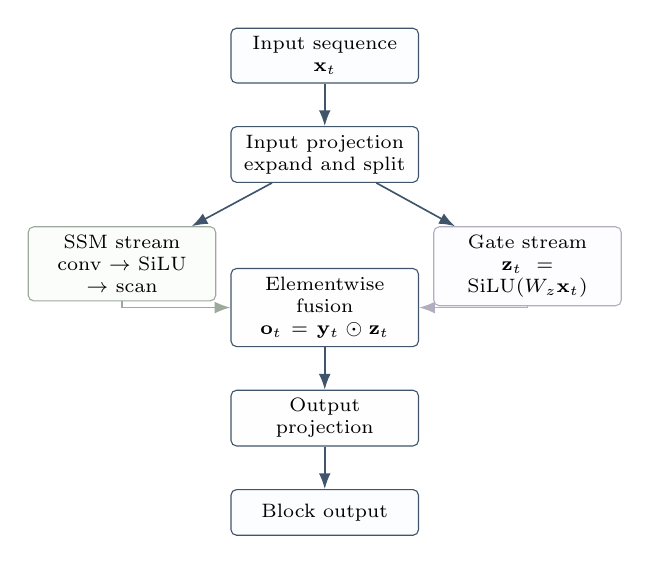
\begin{tikzpicture}[
    node distance=0.54cm and 0.42cm,
    >=Latex,
    arr/.style={->, draw=#1, line width=0.6pt},
    arr/.default={mambaLine},
    block/.style={
        draw=mambaLine,
        rounded corners=2pt,
        fill=white,
        align=center,
        font=\scriptsize,
        inner xsep=4pt,
        inner ysep=3pt,
        minimum height=0.58cm,
        text width=2.10cm
    },
    data/.style={block, fill=mambaBlue!18},
    ssm/.style={block, fill=mambaGreen!14, draw=mambaGreen!70!black},
    gate/.style={block, fill=mambaPurple!12, draw=mambaPurple!75!black},
    op/.style={block, fill=mambaGray!9}
]
\definecolor{mambaBlue}{HTML}{EAF4FF}
\definecolor{mambaGreen}{HTML}{DFF2E1}
\definecolor{mambaPurple}{HTML}{EFE8FF}
\definecolor{mambaGray}{HTML}{F4F6F8}
\definecolor{mambaLine}{HTML}{40556B}

\node[data] (input) {Input sequence\\$\mathbf{x}_t$};
\node[op, below=of input] (proj) {Input projection\\expand and split};
\node[ssm, below left=0.55cm and 0.18cm of proj] (ssmstream) {SSM stream\\conv $\rightarrow$ SiLU $\rightarrow$ scan};
\node[gate, below right=0.55cm and 0.18cm of proj] (gatestream) {Gate stream\\$\mathbf{z}_t=\operatorname{SiLU}(W_z\mathbf{x}_t)$};
\node[op, below=1.08cm of proj] (fusion) {Elementwise fusion\\$\mathbf{o}_t=\mathbf{y}_t\odot\mathbf{z}_t$};
\node[op, below=of fusion] (outproj) {Output projection};
\node[data, below=of outproj] (output) {Block output};

\draw[arr] (input) -- (proj);
\draw[arr] (proj) -- (ssmstream);
\draw[arr] (proj) -- (gatestream);
\draw[arr=mambaGreen!70!black] (ssmstream) |- (fusion);
\draw[arr=mambaPurple!75!black] (gatestream) |- (fusion);
\draw[arr] (fusion) -- (outproj);
\draw[arr] (outproj) -- (output);
\end{tikzpicture}%
}
\end{minipage}
\hfill
\begin{minipage}[t]{0.50\linewidth}
\centering
\textbf{B. Selective SSM component}\\[0.4em]
\resizebox{\linewidth}{!}{%
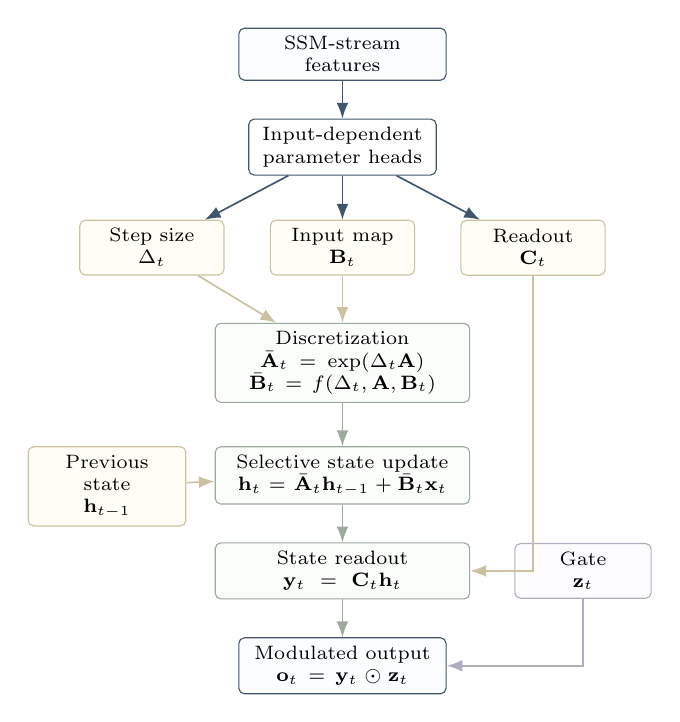
\begin{tikzpicture}[
    node distance=0.48cm and 0.30cm,
    >=Latex,
    arr/.style={->, draw=#1, line width=0.6pt},
    arr/.default={mambaLine},
    block/.style={
        draw=mambaLine,
        rounded corners=2pt,
        fill=white,
        align=center,
        font=\scriptsize,
        inner xsep=4pt,
        inner ysep=3pt,
        minimum height=0.58cm,
        text width=2.10cm
    },
    param/.style={block, fill=mambaGold!18, draw=mambaGold!80!black, text width=1.55cm},
    state/.style={block, fill=mambaGold!16, draw=mambaGold!80!black, text width=1.72cm},
    ssm/.style={block, fill=mambaGreen!14, draw=mambaGreen!70!black, text width=2.95cm},
    gate/.style={block, fill=mambaPurple!12, draw=mambaPurple!75!black, text width=1.45cm},
    data/.style={block, fill=mambaBlue!18, text width=2.35cm}
]
\definecolor{mambaBlue}{HTML}{EAF4FF}
\definecolor{mambaGreen}{HTML}{DFF2E1}
\definecolor{mambaPurple}{HTML}{EFE8FF}
\definecolor{mambaGold}{HTML}{FFF3C9}
\definecolor{mambaLine}{HTML}{40556B}

\node[data] (features) {SSM-stream features};
\node[block, below=of features] (heads) {Input-dependent\\parameter heads};
\node[param, below left=0.56cm and 0.30cm of heads] (delta) {Step size\\$\Delta_t$};
\node[param, below=0.56cm of heads] (bmap) {Input map\\$\mathbf{B}_t$};
\node[param, below right=0.56cm and 0.30cm of heads] (cout) {Readout\\$\mathbf{C}_t$};
\node[ssm, below=0.60cm of bmap] (disc) {Discretization\\$\bar{\mathbf{A}}_t=\exp(\Delta_t\mathbf{A})$\\$\bar{\mathbf{B}}_t=f(\Delta_t,\mathbf{A},\mathbf{B}_t)$};
\node[state, below left=0.55cm and 0.36cm of disc] (prev) {Previous state\\$\mathbf{h}_{t-1}$};
\node[ssm, below=0.55cm of disc] (update) {Selective state update\\$\mathbf{h}_t=\bar{\mathbf{A}}_t\mathbf{h}_{t-1}+\bar{\mathbf{B}}_t\mathbf{x}_t$};
\node[ssm, below=of update] (readout) {State readout\\$\mathbf{y}_t=\mathbf{C}_t\mathbf{h}_t$};
\node[gate, right=0.56cm of readout] (gate) {Gate\\$\mathbf{z}_t$};
\node[data, below=of readout] (modout) {Modulated output\\$\mathbf{o}_t=\mathbf{y}_t\odot\mathbf{z}_t$};

\draw[arr] (features) -- (heads);
\draw[arr] (heads) -- (delta);
\draw[arr] (heads) -- (bmap);
\draw[arr] (heads) -- (cout);
\draw[arr=mambaGold!80!black] (delta) -- (disc);
\draw[arr=mambaGold!80!black] (bmap) -- (disc);
\draw[arr=mambaGreen!70!black] (disc) -- (update);
\draw[arr=mambaGold!80!black] (prev) -- (update);
\draw[arr=mambaGreen!70!black] (update) -- (readout);
\draw[arr=mambaGold!80!black] (cout) |- (readout);
\draw[arr=mambaGreen!70!black] (readout) -- (modout);
\draw[arr=mambaPurple!75!black] (gate) |- (modout);
\end{tikzpicture}%
}
\end{minipage}

    \caption{Mamba block used as the sequence-modeling backbone. Panel A shows the high-level block structure with projection, selective state-space processing, gating, fusion, and output projection. Panel B expands the selective state-space component, where input-dependent parameters control the recurrent update and readout.}
    \label{fig:mamba-arch}
\end{figure}

\subsection{S-Mamba Forecasting Encoder}

Plain Mamba is a sequence block rather than a complete forecasting model.
Given a token sequence $\mathbf{U}\in\mathbb{R}^{B\times T\times d}$, a Mamba block produces another sequence
\begin{equation}
    \mathbf{V}=\mathcal{M}(\mathbf{U})\in\mathbb{R}^{B\times T\times d},
\end{equation}
with the same token axis $T$.
For generic sequence modeling, the token axis is usually time.
S-Mamba changes this setup for forecasting by using reversible window normalization and inverted variable tokens.

For an input window $\mathbf{X}\in\mathbb{R}^{B\times L\times C}$, S-Mamba first applies reversible normalization:
\begin{equation}
    \mu_{b,c}
    =
    \frac{1}{L}\sum_{t=1}^{L}X_{b,t,c},
    \qquad
    \sigma_{b,c}
    =
    \sqrt{
        \frac{1}{L}\sum_{t=1}^{L}(X_{b,t,c}-\mu_{b,c})^2 + \epsilon
    },
\end{equation}
\begin{equation}
    Z_{b,t,c}
    =
    \frac{X_{b,t,c}-\mu_{b,c}}{\sigma_{b,c}}.
\end{equation}
Each variable history is then embedded as one token:
\begin{equation}
    \mathbf{e}_{b,c}
    =
    W_{\mathrm{emb}}\mathbf{z}_{b,:,c}+ \mathbf{b}_{\mathrm{emb}},
    \qquad
    \mathbf{E}\in\mathbb{R}^{B\times C\times d_{\mathrm{model}}},
\end{equation}
where $\mathbf{z}_{b,:,c}\in\mathbb{R}^{L}$ is the normalized history of variable $c$.
Thus, S-Mamba scans along variable tokens whose features are full lookback histories, rather than scanning directly along time tokens.

Each encoder layer is bidirectional.
Let $\mathbf{E}^{(\ell-1)}$ be the input to layer $\ell$.
The forward and backward Mamba branches are
\begin{equation}
    \overrightarrow{\mathbf{H}}^{(\ell)}
    =
    \mathcal{M}_{f}^{(\ell)}(\mathbf{E}^{(\ell-1)}),
    \qquad
    \overleftarrow{\mathbf{H}}^{(\ell)}
    =
    \operatorname{rev}
    \left(
    \mathcal{M}_{b}^{(\ell)}
    \left(
    \operatorname{rev}(\mathbf{E}^{(\ell-1)})
    \right)
    \right),
\end{equation}
and the two directions are added:
\begin{equation}
    \mathbf{U}^{(\ell)}
    =
    \overrightarrow{\mathbf{H}}^{(\ell)}
    +
    \overleftarrow{\mathbf{H}}^{(\ell)}.
\end{equation}
The implemented layer then applies residual connections, layer normalization, and a feed-forward network:
\begin{equation}
    \tilde{\mathbf{E}}^{(\ell)}
    =
    \operatorname{LN}_{1}
    \left(
    \mathbf{E}^{(\ell-1)}+\mathbf{U}^{(\ell)}
    \right),
\end{equation}
\begin{equation}
    \mathbf{E}^{(\ell)}
    =
    \operatorname{LN}_{2}
    \left(
    \tilde{\mathbf{E}}^{(\ell)}+
    \operatorname{FFN}
    \left(
    \tilde{\mathbf{E}}^{(\ell)}
    \right)
    \right).
\end{equation}
After the final encoder layer, each variable token is projected to the horizon:
\begin{equation}
    \mathbf{P}_{b,c,:}
    =
    W_{\mathrm{out}}\mathbf{E}^{(L_e)}_{b,c,:}
    + \mathbf{b}_{\mathrm{out}},
    \qquad
    \mathbf{P}\in\mathbb{R}^{B\times C\times H}.
\end{equation}
The forecast is permuted back to the time-major layout and de-normalized:
\begin{equation}
    \hat{Y}_{b,h,c}
    =
    \sigma_{b,c} P_{b,c,h} + \mu_{b,c}.
\end{equation}

Figure~\ref{fig:s-mamba-encoder} summarizes the S-Mamba forecasting encoder.

\begin{figure}[t]
    \centering
    \centering
\resizebox{0.72\linewidth}{!}{%
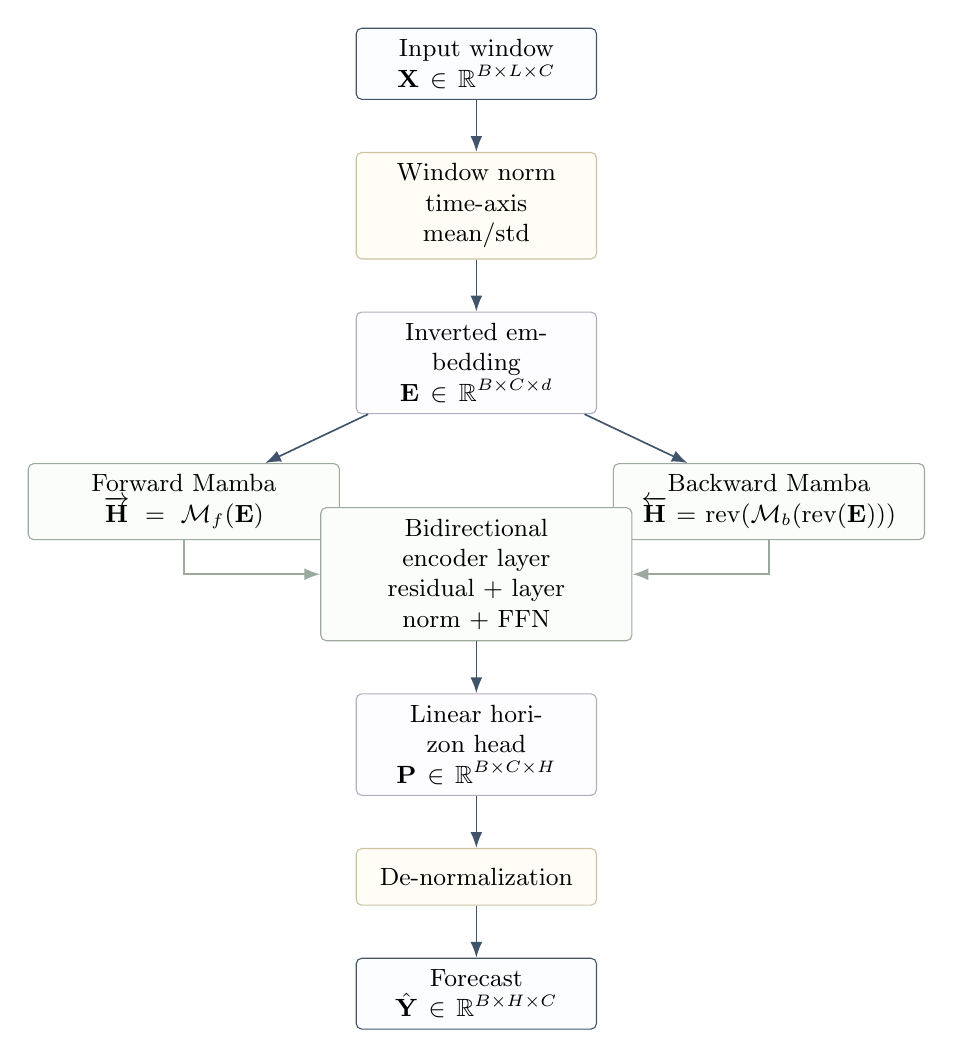
\begin{tikzpicture}[
    node distance=0.66cm and 0.42cm,
    >=Latex,
    arr/.style={->, draw=#1, line width=0.6pt},
    arr/.default={mLine},
    block/.style={
        draw=mLine,
        rounded corners=2pt,
        fill=white,
        align=center,
        font=\small,
        inner xsep=5pt,
        inner ysep=4pt,
        minimum height=0.72cm,
        text width=2.70cm
    },
    data/.style={block, fill=mBlue!16},
    norm/.style={block, fill=mGold!16, draw=mGold!80!black},
    enc/.style={block, fill=mGreen!14, draw=mGreen!70!black, text width=3.60cm},
    proj/.style={block, fill=mPurple!12, draw=mPurple!75!black}
]
\definecolor{mBlue}{HTML}{EAF4FF}
\definecolor{mGreen}{HTML}{DFF2E1}
\definecolor{mPurple}{HTML}{EFE8FF}
\definecolor{mGold}{HTML}{FFF3C9}
\definecolor{mLine}{HTML}{40556B}

\node[data] (input) {Input window\\$\mathbf{X}\in\mathbb{R}^{B\times L\times C}$};
\node[norm, below=of input] (norm) {Window norm\\time-axis mean/std};
\node[proj, below=of norm] (embed) {Inverted embedding\\$\mathbf{E}\in\mathbb{R}^{B\times C\times d}$};
\node[enc, below left=0.62cm and 0.20cm of embed] (forward) {Forward Mamba\\$\overrightarrow{\mathbf{H}}=\mathcal{M}_f(\mathbf{E})$};
\node[enc, below right=0.62cm and 0.20cm of embed] (backward) {Backward Mamba\\$\overleftarrow{\mathbf{H}}=\operatorname{rev}(\mathcal{M}_b(\operatorname{rev}(\mathbf{E})))$};
\node[enc, below=1.18cm of embed] (fusion) {Bidirectional encoder layer\\residual + layer norm + FFN};
\node[proj, below=of fusion] (head) {Linear horizon head\\$\mathbf{P}\in\mathbb{R}^{B\times C\times H}$};
\node[norm, below=of head] (denorm) {De-normalization};
\node[data, below=of denorm] (forecast) {Forecast\\$\hat{\mathbf{Y}}\in\mathbb{R}^{B\times H\times C}$};

\draw[arr] (input) -- (norm);
\draw[arr] (norm) -- (embed);
\draw[arr] (embed) -- (forward);
\draw[arr] (embed) -- (backward);
\draw[arr=mGreen!70!black] (forward) |- (fusion);
\draw[arr=mGreen!70!black] (backward) |- (fusion);
\draw[arr] (fusion) -- (head);
\draw[arr] (head) -- (denorm);
\draw[arr] (denorm) -- (forecast);
\end{tikzpicture}%
}

    \caption{S-Mamba forecasting encoder: reversible normalization, inverted variable-token embedding, bidirectional Mamba encoding, horizon projection, and de-normalization back to the original price scale.}
    \label{fig:s-mamba-encoder}
\end{figure}

\subsection{Nonstationarity Statistics}

The NS-Mamba variants expose window statistics to two different modules.
Adaptive normalization uses raw window statistics to generate affine parameters, while shift-aware gates use standardized statistics to produce fusion weights.
Both are computed from the raw input window before normalization.

For adaptive normalization, the implementation constructs a ten-dimensional statistic vector for each sample and variable:
\begin{equation}
    \psi_{b,c}
    =
    [
    \mu_{b,c},
    \sigma_{b,c},
    X_{b,1,c},
    X_{b,L,c},
    \mu^{r}_{b,c},
    \sigma^{r}_{b,c},
    X_{b,L,c}-X_{b,1,c},
    \min_t X_{b,t,c},
    \max_t X_{b,t,c},
    \nu_{b,c}
    ],
\end{equation}
where $\mu_{b,c}$ and $\sigma_{b,c}$ are full-window mean and standard deviation, $\mu^{r}_{b,c}$ and $\sigma^{r}_{b,c}$ are computed on the most recent segment of the window, and $\nu_{b,c}$ is the standard deviation of first differences.
The recent segment length is controlled by the hyperparameter \texttt{ns\_recent\_ratio}, with default value 0.25.

For shift-aware fusion, the implementation uses an eight-dimensional standardized feature vector:
\begin{equation}
    \phi_{b,c}
    =
    [
    \delta_{\mu},
    \delta_{\sigma},
    s,
    \bar{\nu},
    \delta_{\nu},
    r,
    z_L,
    z_1
    ]_{b,c}.
\end{equation}
Let $\sigma_{b,c}^{+}=\sigma_{b,c}+\epsilon$.
The entries are
\begin{align}
    \delta_{\mu}
    &=
    \frac{\mu^{r}_{b,c}-\mu_{b,c}}{\sigma_{b,c}^{+}},
    &
    \delta_{\sigma}
    &=
    \log
    \frac{\sigma^{r}_{b,c}+\epsilon}{\sigma_{b,c}^{+}},
    \\
    s
    &=
    \frac{X_{b,L,c}-X_{b,1,c}}{\sigma_{b,c}^{+}},
    &
    \bar{\nu}
    &=
    \frac{\nu_{b,c}}{\sigma_{b,c}^{+}},
    \\
    \delta_{\nu}
    &=
    \log
    \frac{\nu^{r}_{b,c}+\epsilon}{\nu_{b,c}+\epsilon},
    &
    r
    &=
    \frac{\max_t X_{b,t,c}-\min_t X_{b,t,c}}{\sigma_{b,c}^{+}},
    \\
    z_L
    &=
    \frac{X_{b,L,c}-\mu_{b,c}}{\sigma_{b,c}^{+}},
    &
    z_1
    &=
    \frac{X_{b,1,c}-\mu_{b,c}}{\sigma_{b,c}^{+}}.
\end{align}
Here $\nu^{r}_{b,c}$ is the recent-segment standard deviation of first differences.
The fusion gates project $\phi_{b,c}$ into the hidden dimension and combine it with the hidden representation when one is available.
When the number of statistic tokens does not match the number of target tokens, the statistic context is averaged over variables and broadcast to the required token count.

\subsection{Adaptive Normalization}

Adaptive normalization replaces fixed reversible normalization with a learned affine transformation conditioned on $\psi_{b,c}$.
For each variable token, an MLP maps $\psi_{b,c}$ to raw affine parameters, and the bounded transformation is
\begin{equation}
    \gamma_{b,c}
    =
    1 + a \tanh(g_{\gamma}(\psi_{b,c})),
    \qquad
    \beta_{b,c}
    =
    a \tanh(g_{\beta}(\psi_{b,c})),
\end{equation}
where $a$ is the adaptive-scale hyperparameter.
The normalized input is
\begin{equation}
    \tilde{X}_{b,t,c}
    =
    \gamma_{b,c}
    \frac{X_{b,t,c}-\mu_{b,c}}{\sigma_{b,c}+\epsilon}
    +
    \beta_{b,c}.
\end{equation}
The same cached $\gamma_{b,c}$, $\beta_{b,c}$, $\mu_{b,c}$, and $\sigma_{b,c}$ are used to invert the transformation at the output:
\begin{equation}
    \hat{Y}_{b,h,c}
    =
    \left(
    \frac{\tilde{Y}_{b,h,c}-\beta_{b,c}}{\gamma_{b,c}}
    \right)
    (\sigma_{b,c}+\epsilon)
    +
    \mu_{b,c}.
\end{equation}

\subsection{Series Decomposition}

The decomposition module separates the normalized window into low-frequency, medium-frequency, and residual components using moving averages.
Let $\operatorname{MA}_{m}(\cdot)$ denote a centered moving average with boundary replication and window size $m$.
The implementation computes
\begin{align}
    \mathbf{Z}^{\mathrm{tr}}
    &=
    \operatorname{MA}_{m}(\mathbf{Z}),
    \\
    \mathbf{R}^{0}
    &=
    \mathbf{Z}-\mathbf{Z}^{\mathrm{tr}},
    \\
    \mathbf{Z}^{\mathrm{mf}}
    &=
    \operatorname{MA}_{m}(\mathbf{R}^{0}),
    \\
    \mathbf{Z}^{\mathrm{re}}
    &=
    \mathbf{R}^{0}-\mathbf{Z}^{\mathrm{mf}}.
\end{align}
The superscripts denote low-frequency trend-like, medium-frequency, and residual components.
This decomposition is an architectural bias rather than a claim that GLD prices are generated by a perfect additive seasonal process.

\subsection{Shift-Aware Fusion}

Shift-aware gates use $\phi_{b,c}$ to control either branch fusion or hidden-state interpolation.
For decomposition branches with horizon-level outputs $\mathbf{U}_q\in\mathbb{R}^{B\times C\times H}$, where $q\in\{\mathrm{tr},\mathrm{mf},\mathrm{re}\}$, the branch gate computes
\begin{equation}
    \boldsymbol{\alpha}_{b,c,:,h}
    =
    \operatorname{softmax}_{q}
    \left(
    g_{\alpha}(\phi_{b,c})
    \right),
\end{equation}
and fuses the branch outputs as
\begin{equation}
    \mathbf{U}_{b,c,h}
    =
    \sum_q \alpha_{b,c,q,h}\mathbf{U}_{q,b,c,h}.
\end{equation}
The same gate class is also used for scale fusion in the multi-scale models, where the softmax dimension ranges over temporal scales rather than decomposition components.
When no decomposition branch is present, a sigmoid gate can interpolate between the encoded hidden state and the input embedding before horizon projection:
\begin{equation}
    \tilde{\mathbf{E}}
    =
    \mathbf{G}\odot \mathbf{E}_{\mathrm{enc}}
    +
    (1-\mathbf{G})\odot \mathbf{E}_{\mathrm{in}}.
\end{equation}

\subsection{Variant Definitions}

The Mamba-family variant names encode which modules are active.
\textbf{A} denotes adaptive normalization, \textbf{D} denotes decomposition, and \textbf{G} denotes shift-aware gated fusion.
\textbf{M} denotes multi-scale temporal branches, \textbf{S} denotes an NLinear-style residual skip, and \textbf{P} denotes patch-temporal Mamba branches.
All variants produce forecasts with shape $\mathbb{R}^{B \times H \times C}$ and use reversible output scaling when normalization is enabled.

Let $\mathcal{N}(\cdot)$ denote standard reversible normalization and $\mathcal{F}_{\theta}(\cdot)$ denote one inverted S-Mamba forecasting branch.
The S-Mamba baseline is
\begin{equation}
    \hat{\mathbf{Y}}_{\mathrm{S}}
    =
    \mathcal{N}^{-1}
    \left(
    \mathcal{F}_{\theta}(\mathcal{N}(\mathbf{X}))
    \right).
\end{equation}
NS-Mamba-A replaces $\mathcal{N}$ with adaptive normalization.
NS-Mamba-D applies standard reversible normalization, decomposes the normalized signal, and sums three independently encoded component forecasts:
\begin{equation}
    \hat{\mathbf{Y}}_{\mathrm{D}}
    =
    \mathcal{N}^{-1}
    \left(
    \sum_{q \in \{\mathrm{tr},\mathrm{mf},\mathrm{re}\}}
    \mathcal{F}_{\theta_q}(\mathbf{Z}^{q})
    \right).
\end{equation}
NS-Mamba-AD combines adaptive normalization with decomposition, and NS-Mamba-ADG adds the shift-aware branch gate.

The MS-Mamba family adds temporal scale branches.
Let $\mathcal{P}_{s}(\cdot)$ be average-pooling downsampling by scale $s$, and let $\mathcal{S}$ be a set of scales such as $\{1,2,4\}$.
For a decomposition-enabled multi-scale model, each scale produces
\begin{equation}
    \mathbf{U}_{s}
    =
    \sum_{q \in \{\mathrm{tr},\mathrm{mf},\mathrm{re}\}}
    \mathcal{F}_{\theta_{s,q}}
    \left(
    \mathcal{P}_{s}(\mathbf{Z}^{q})
    \right).
\end{equation}
MS-Mamba-MD uses mean scale fusion:
\begin{equation}
    \hat{\mathbf{Y}}_{\mathrm{MD}}
    =
    \mathcal{N}^{-1}
    \left(
    \frac{1}{|\mathcal{S}|}
    \sum_{s \in \mathcal{S}}
    \mathbf{U}_{s}
    \right),
\end{equation}
while MS-Mamba-MDG replaces the mean with a shift-aware softmax over scales.
MS-Mamba-M and MS-Mamba-MG are the corresponding multi-scale variants without decomposition.

MS-Mamba-MDS adds a last-value residual linear skip:
\begin{equation}
    \mathbf{U}_{\mathrm{skip}}
    =
    \mathbf{x}_{L}
    +
    \mathbf{W}_{\mathrm{skip}}
    (\mathbf{Z}-\mathbf{x}_{L}),
    \qquad
    \hat{\mathbf{Y}}_{\mathrm{MDS}}
    =
    \mathcal{N}^{-1}
    \left(
    \lambda \mathbf{U}_{\mathrm{MD}}
    +
    (1-\lambda)\mathbf{U}_{\mathrm{skip}}
    \right),
\end{equation}
where $\lambda=\sigma(\rho)$ is learned.
PMS-Mamba replaces inverted variable-token branches with patch-temporal Mamba branches.
For patch length $p$ and stride $r$, a scale branch forms patch tokens
\begin{equation}
    \mathbf{e}_{j}^{(s)}
    =
    \mathbf{W}_{p}
    \operatorname{vec}
    \left(
    \mathcal{P}_{s}(\mathbf{Z})_{j:j+p-1}
    \right),
\end{equation}
then applies Mamba over the patch index $j$.
PMS-Mamba-PD is the patch-temporal counterpart of MS-Mamba-MD.

\begin{table}[t]
\centering
\caption{Meaning of the Mamba-family variant names used in this manuscript.}
\label{tab:mamba-variant-meaning}
{\small
\begin{tabular}{p{0.19\linewidth}p{0.27\linewidth}p{0.16\linewidth}p{0.26\linewidth}}
\toprule
Variant & Active modules & Fusion & Purpose \\
\midrule
NS-Mamba-A & Adaptive norm & Single path & Test learned normalization \\
NS-Mamba-D & Decomposition & Sum & Test component separation \\
NS-Mamba-AD & Adaptive norm + decomposition & Sum & Combine A and D \\
NS-Mamba-ADG & Adaptive norm + decomposition & Shift gate & Test gated component fusion \\
MS-Mamba-M & Multi-scale & Mean & Test temporal scales alone \\
MS-Mamba-MG & Multi-scale & Shift gate & Test gated scale fusion \\
MS-Mamba-MD & Multi-scale + decomposition & Mean & Promoted Mamba model \\
MS-Mamba-MDG & Multi-scale + decomposition & Shift gate & Test gated multi-scale decomposition \\
MS-Mamba-MDS & Multi-scale + decomposition + skip & Mean + skip & Test NLinear-style residual path \\
PMS-Mamba-PD & Patch Mamba + decomposition & Mean & Test patch Mamba \\
\bottomrule
\end{tabular}
}
\end{table}

\subsection{Forecast Head and Loss}

The forecast head projects the final hidden representation to $H$ future values.
The training objective is mean squared error over the forecast horizon:
\begin{equation}
    \mathcal{L}
    =
    \frac{1}{BHC_o}
    \sum_{b=1}^{B}
    \sum_{h=1}^{H}
    \sum_{c=1}^{C_o}
    \left(
    \hat{Y}_{b,h,c} - Y_{b,h,c}
    \right)^2.
\end{equation}
Inverse transformation is enabled by default in the reported GLD runs, so saved predictions, targets, and metrics are reported on the original GLD price scale unless a run uses \texttt{--no-inverse}.

\section{Experimental Setup}

\subsection{Dataset}

The initial dataset is GLD daily data stored at \texttt{data/GLD/GLD.csv}.
The target column is \texttt{close}.
The first experimental phase uses single-target forecasting.
Future extensions may add more financial or macroeconomic variables, but those are outside the current baseline protocol.

\subsection{Data Splits}

The repository uses the standard custom-data split from the forecasting codebase.
The validation and test windows use historical lookback context from the previous split to construct the input sequence.
This is a common forecasting implementation detail, but it should be reported clearly because the input context for validation and test includes observations before the split boundary.

\subsection{Baseline Models}

The core baseline set is:
\begin{itemize}
    \item S\_Mamba;
    \item Transformer;
    \item Informer;
    \item Reformer;
    \item Autoformer;
    \item iTransformer.
\end{itemize}
Optional Mamba-augmented variants will be reported separately if they are included.
The clean baselines should not be tuned independently after the shared setting is locked.

\subsection{Shared Configuration}

S\_Mamba calibration selected Setting A as the locked baseline configuration:
\begin{center}
\begin{tabular}{ll}
\toprule
Parameter & Value \\
\midrule
Lookback length & 360 \\
Label length & 180 \\
Prediction length & horizon-specific \\
Model dimension & 64 \\
Feed-forward dimension & 128 \\
Encoder layers & 2 \\
Batch size & 16 \\
Target & \texttt{close} \\
Output scale & original price scale \\
\bottomrule
\end{tabular}
\end{center}
All suitable models will use this configuration.
If a model cannot run under this setting, the failure will be recorded rather than changing only that model's hyperparameters.

\subsection{Metrics and Logging}

The primary manuscript metrics are RMSE and MAE.
MSE, MAPE, and MSPE are also saved when available.
Training, validation, and test metrics are logged to TensorBoard.
Final arrays are saved as \texttt{pred.npy}, \texttt{true.npy}, and \texttt{metrics.npy}, with run metadata stored in \texttt{meta.json}.
The completed GLD baseline sweep contains 72 finished runs, corresponding to 6 models across 12 horizons.

\section{Interim Results}

\subsection{Selection-Safe Evidence}

The evidence presently available supports the intended nonstationary setting but not a forecasting-performance conclusion.
Across all four training targets, the level ADF test fails to reject a unit root while the level KPSS test rejects trend stationarity at its reported lower $p$-value bound (Table~\ref{tab:selection-safe-diagnostics}).
This concordance is not treated as proof that every series follows an integrated process; it establishes that a stationary-level assumption is not an adequate common description of the training panels.

The held-out validation interval differs visibly from training (Figure~\ref{fig:financial-nonstationarity}).
Foreign exchange and Treasury yields shift downward by 1.294 and 0.512 training standard deviations, respectively, whereas GLD shifts upward by 1.708 standard deviations.
BTCUSDT exhibits the largest shift: its validation mean is 7.750 training standard deviations above the training mean, its level standard deviation is 3.669 times the training value, and its first-difference standard deviation is 4.521 times the training value.
These quantities justify evaluating distribution-shift-sensitive designs, but they do not predict which model will perform best in the untouched final period.

The MS tasks also face changing cross-series structure.
The maximum absolute change from training to validation in a feature--target first-difference correlation is 0.268 for foreign exchange, 0.026 for yields, 0.323 for cross assets, and 0.106 for cryptoassets.
Consequently, an MS improvement cannot be assumed merely because additional histories are supplied; the paired S/MS comparison is required.

\subsection{Locked Outcome Status}

Table~\ref{tab:evidence-status} records the evidence boundary for this manuscript version.
Source retrieval, preprocessing, checksums, fixed splits, selection-safe diagnostics, and validation-only hyperparameter selection are complete.
The frozen selection audit has passed; the final neural matrix, statistical-reference forecasts, bootstrap contrasts, and full-period diagnostics have not been generated because the protected final period has not been opened.
The result generator is designed to fail unless all required artifacts match the frozen protocol and data hashes.

\begin{table}[H]
\centering
\caption{Evidence status for the interim manuscript. ``Locked'' means that the workflow requires an explicit gate and preceding completeness audit before reading final-period targets.}
\label{tab:evidence-status}
{\small
\begin{tabular}{>{\raggedright\arraybackslash}p{0.29\linewidth}>{\raggedright\arraybackslash}p{0.23\linewidth}>{\raggedright\arraybackslash}p{0.38\linewidth}}
\toprule
Evidence component & Status & Admissible use in this version \\
\midrule
Source and processed-data manifests & Complete & Dataset provenance and counts \\
Training/validation diagnostics & Complete & Selection-safe characterization \\
Validation-only model selection & Complete (audit passed) & Configuration freeze only; no ranking claim \\
2023--2026 neural evaluation & Locked & None \\
Statistical-reference evaluation & Blocked by neural matrix & None \\
Bootstrap and regime outcome analysis & Not generated & None \\
\bottomrule
\end{tabular}
}
\end{table}

\subsection{Prespecified Final Reporting}

After the protected evaluation is unlocked and validated, the final paper will report every task separately.
The primary table will contain balanced path RMSSE for last-value, the validation-selected non-Mamba comparator, S-Mamba, and the three proposed Mamba variants; neural entries will be mean $\pm$ standard deviation over five seeds.
Horizon-specific path and terminal metrics, random-walk-with-drift, ARIMA, and VAR-difference estimates will be retained in generated supplementary tables rather than selectively omitted.

Claims of improvement will require more than the smallest point estimate.
They will be based on paired origin-level loss differences, 95\% moving-block bootstrap intervals, and Holm-adjusted $p$-values for the prespecified contrasts.
The S/MS analysis will report signed differences for the same panel, model, and horizon.
Regime results will remain secondary, and return forecasts will be labeled robustness analyses performed only after completion of the level benchmark.

\section{Discussion and Limitations}

The selection-safe evidence confirms that the benchmark poses the intended problem: persistent financial levels are accompanied by substantial temporal changes in location, scale, volatility, and, for some panels, feature--target correlations.
The size and direction of these changes vary sharply across panels.
This heterogeneity is precisely why the study is organized around task-level estimates and paired comparisons rather than a single rank averaged across unrelated units.

Several outcome interpretations are fixed in advance.
First, a neural model is not considered useful merely because it outperforms another neural architecture; performance relative to last-value and other statistical references is central.
Second, a favorable result on one panel or horizon does not establish general Mamba superiority.
Third, an MS advantage indicates predictive value from the supplied panel histories under this protocol, not a causal cross-market mechanism.
Fourth, level-forecast accuracy is not evidence of profitable trading, market inefficiency, directional accuracy, calibrated risk, or robustness to transaction costs.

The benchmark improves on the legacy development experiments by using a newly frozen final period, fixed task definitions, equal trial counts, five neural seeds, explicit statistical references, and dependence-aware paired resampling.
The protocol and processed-data hashes are checked at every transition, and final manuscript generation is blocked until the complete matrix is available.
These controls reduce opportunities for selective reporting, but they do not eliminate all researcher degrees of freedom.
The model families and their search spaces reflect prior development, and the proposed Mamba variants are not accompanied by a full factorial ablation that isolates tokenization, decomposition, scale construction, and parameter count.

The data design also has limitations.
Four panels cannot represent all financial markets, frequencies, or institutional regimes.
Complete-case intersection removes imputation assumptions but changes each panel's observation calendar and may privilege dates on which every constituent market reports.
The study uses one fixed final interval rather than multiple historical backtests, and the shortest cryptoasset training segment contains 973 observations.
The final period may therefore provide a demanding distribution shift without supporting broad temporal generalization.

Statistical uncertainty remains conditional on the implemented resampling design.
Forecast origins overlap, losses at different horizons are related, and five neural seeds quantify only part of optimization variability.
The moving-block bootstrap preserves local origin dependence approximately; its block-length rule is prespecified rather than estimated for each series.
Holm adjustment is applied within each task--proposal--comparator horizon family, not across every exploratory quantity in the paper.
Regime estimates are secondary and may have unequal origin counts.

The statistical references are intentionally practical rather than exhaustive.
ARIMA and VAR orders are selected on the training period; coefficients are estimated once from the full pre-test history, remain fixed during final evaluation, and observed values update the forecasting state sequentially.
In contrast, neural weights are estimated from training observations while validation controls early stopping.
This asymmetric use of validation values gives the statistical references a conservative information advantage and must be retained when interpreting neural-to-statistical differences.
More elaborate financial-econometric specifications, probabilistic forecasts, and models of conditional variance are outside the primary comparison.
Specialist financial-econometrics review is therefore warranted before submission, particularly for any interpretation beyond point-forecast accuracy.

Finally, this interim version has no confirmatory performance result.
Validation scores are model-selection evidence and will not be substituted for test outcomes.
The discussion must be revised after the final matrix is complete, including explicit reporting of negative or null results.
Dataset redistribution terms, a citable code archive, author contributions, funding, competing interests, and venue-specific AI-use disclosure also require accountable author confirmation before submission.

\section{Conclusion}

This study describes completed single-seed evaluations of four Mamba variants, ten tuned neural baselines, and last-value forecasts on two univariate financial level series.
On GLD, PMS-Mamba-PD has the lowest observed balanced RMSSE at 14.74, compared with TimesNet at 15.66 and last-value at 17.07.
On Exchange, last-value is lowest at 6.26, ahead of S-Mamba at 6.29 and PatchTST at 6.37.

The benchmark therefore does not establish general Mamba superiority.
Its defensible result is narrower: the tested patch-temporal Mamba configuration is competitive on the current GLD period, while persistence remains the stronger reference on Exchange.
Because architecture development used prior GLD test outcomes, search budgets differ, training uses one seed, forecast windows overlap, and no inferential intervals are available, all reported differences are descriptive.
An untouched evaluation period, equal-compute tuning, repeated seeds, dependence-aware uncertainty, controlled ablations, and broader datasets are required before confirmatory or mechanism-level claims can be made.

\appendix
\section{Theoretical Properties}
\label{app:theory}
\subsection{Proof of Proposition~\ref{prop:single-token}}

The inverted embedding constructs one token for each of the $C$ input variables and passes the resulting sequence to the bidirectional Mamba encoder.
When $C=1$, the encoder sequence is $(\mathbf{e}_1)$.
There is no pair of distinct temporal token indices $j-1$ and $j$ at which a transition can be evaluated.
The output can still depend on the complete history because $\mathbf{e}_1$ is computed from that history, but the state-space block has no recurrence across temporal tokens.
\hfill$\square$

\subsection{Proof of Proposition~\ref{prop:additive}}

By construction, $\mathbf{D}=\mathbf{Z}-\mathbf{T}$ and $\mathbf{R}=\mathbf{D}-\mathbf{S}$.
Therefore,
\begin{equation}
    \mathbf{T}+\mathbf{S}+\mathbf{R}
    =\mathbf{T}+\mathbf{S}+(\mathbf{Z}-\mathbf{T})-\mathbf{S}
    =\mathbf{Z}.
\end{equation}
The result holds independently of the moving-average width and boundary replication rule.
\hfill$\square$

\subsection{Proof of Proposition~\ref{prop:stable-fusion}}

Every coordinate of $\mathcal{P}_s(\mathbf{U})$ is an arithmetic mean of a nonempty set of input coordinates.
For any pooled window $I$,
\begin{equation}
    \left|\frac{1}{|I|}\sum_{i\in I}(U_i-V_i)\right|
    \leq \frac{1}{|I|}\sum_{i\in I}|U_i-V_i|
    \leq \|\mathbf{U}-\mathbf{V}\|_{\infty}.
\end{equation}
Taking the maximum over pooled coordinates yields the pooling inequality.
For fixed forecasts $\widetilde{Y}^{(s)}$, mean fusion is a convex combination with weights $1/|\mathcal{S}|$.
Each fused coordinate therefore lies in the interval spanned by the corresponding scale-specific coordinates.
\hfill$\square$

\section{Frozen Protocol and Reproducibility Details}
\subsection{Frozen protocol}
\label{app:frozen-protocol}

\begin{table}[H]
\centering
\caption{Controlling protocol fields.}
\label{tab:frozen-protocol}
\begin{tabular}{ll}
\toprule
Field & Frozen value \\
\midrule
Version & \texttt{financial\_confirmatory\_v1} \\
Frozen on & 2026-07-25 \\
Data cutoff & 2026-06-30 \\
Train / validation / test & through 2020 / 2021--2022 / 2023--2026-06 \\
Horizons & 1, 5, 20, 60, 120, 252 observations \\
Calibration horizons & 5, 60, 252 observations \\
Trials / full replays & 12 effective trials / top 3 completed trials \\
Training cap / patience & 10 epochs / 3 epochs \\
HPO sampler seed & 20260725 \\
Final neural seeds & 2023, 2024, 2025, 2026, 2027 \\
Bootstrap & 10,000 circular moving-block replicates; seed 20260725 \\
\bottomrule
\end{tabular}
\end{table}

The eight task identifiers are listed by panel in Table~\ref{tab:task-identifiers}.
\begin{table}[H]
\centering
\caption{Paired task identifiers.}
\label{tab:task-identifiers}
\begin{tabular}{lll}
\toprule
Panel & S task & MS task \\
\midrule
Foreign exchange & \texttt{financial\_fx\_s} & \texttt{financial\_fx\_ms} \\
Treasury yields & \texttt{financial\_yields\_s} & \texttt{financial\_yields\_ms} \\
Cross asset & \texttt{financial\_cross\_asset\_s} & \texttt{financial\_cross\_asset\_ms} \\
Cryptoasset & \texttt{financial\_crypto\_s} & \texttt{financial\_crypto\_ms} \\
\bottomrule
\end{tabular}
\end{table}
Every manifest entry stores its processed-data hash, the protocol hash, fixed split dates, target, input/output channel counts, horizon suite, and term groups.

\subsection{Neural search spaces}

The following values are categorical choices, not continuous ranges.
All models use two encoder layers, dropout 0.1, and label length $L/2$ unless the implementation ignores a field.
The common Mamba space is $L\in\{16,32,64,96,128,192,256,320,384\}$, $d_{\mathrm{model}}\in\{64,128\}$, $d_{\mathrm{ff}}\in\{128,256\}$, state dimension $\in\{16,32\}$, moving-average window $\in\{13,25,49\}$, learning rate $\in\{5\times10^{-5},10^{-4},2\times10^{-4},3\times10^{-4}\}$, and batch size 16.
S-Mamba adds no variant-specific choice.
NS-Mamba-D fixes standard rather than adaptive normalization, activates decomposition, and disables shift gating.
MS-Mamba-MD chooses scales from $\{1,2,4\}$, $\{1,2,4,8\}$, $\{1,3,6\}$, or $\{1,4,8\}$; it fixes decomposition on, mean scale fusion, and no linear skip.
PMS-Mamba-PD chooses $\{1,2,4\}$ or $\{1,2,4,8\}$ and a patch-length/stride pair from $(8,4)$, $(8,8)$, $(16,4)$, or $(16,8)$; infeasible scaled patch layouts are rejected before training.

\begin{table*}[t]
\centering
\caption{Non-Mamba categorical search spaces. ``LR'' denotes learning rate and ``BS'' batch size.}
\label{tab:baseline-search-spaces}
\resizebox{\textwidth}{!}{%
\begin{tabular}{llllll}
\toprule
Model & Lookback $L$ & Width choices & LR & BS & Specific choices \\
\midrule
DLinear & 96, 192, 256 & -- & 0.003, 0.005 & 32, 64 & Moving average 13, 25; shared channels \\
NLinear & 64, 192, 320, 384 & -- & 0.005, 0.01 & 32, 64 & Shared channels \\
PatchTST & 128, 256, 320 & $d_m$: 128, 256; $d_{ff}$: 512, 2048 & 0.0002, 0.0003, 0.0005 & 16, 32 & Patch/stride: 16/8, 24/12, 32/16 \\
TimesNet & 128, 256, 320 & $d_m$: 32, 64; $d_{ff}$: 128, 256 & 0.0001, 0.0002, 0.0003 & 16, 32 & Top-$k=5$; kernels 6, 8 \\
iTransformer & 128, 192, 256 & $d_m$: 128, 256; $d_{ff}$: 256, 512 & 0.0001, 0.0002, 0.0003 & 16 & Reversible normalization on \\
\bottomrule
\end{tabular}%
}
\end{table*}

Optuna uses TPE with the frozen sampler seed and a median pruner with four startup trials, one warm-up step, and one-step intervals.
Interrupted \texttt{RUNNING} trials are marked \texttt{FAIL} on recovery.
The fixed budget counts \texttt{COMPLETE} and \texttt{PRUNED} trials; failed trials do not consume it.
Only completed trials can enter the top-three full validation replay.

\subsection{Reference-model specification}

Last-value and random-walk-with-drift have no fitted hyperparameters.
ARIMA searches $d\in\{0,1\}$ and $p,q\in\{0,1,2,3\}$ on the training target and selects minimum AIC; ARIMA$(0,0,0)$ is excluded.
A time trend is used for $d=1$, and a constant plus trend is used for $d=0$.
VAR-difference is available only for MS tasks and selects lags 1--10 by minimum training BIC with constant and trend.
After order or lag selection, coefficients are estimated once using all observations before the test boundary.
At each final origin, ARIMA state and VAR lagged differences use observations available up to that origin, while fitted coefficients remain fixed.

\subsection{Artifact gates and regeneration}

The complete workflow is executed in the Anaconda environment with:
\begin{verbatim}
conda run --no-capture-output -n mamba python \
  scripts/financial/run_financial_benchmark.py --stage hpo
conda run --no-capture-output -n mamba python \
  scripts/financial/run_financial_benchmark.py --stage selection
conda run --no-capture-output -n mamba python \
  scripts/financial/run_financial_benchmark.py --stage final --unlock-test
conda run --no-capture-output -n mamba python \
  scripts/financial/run_statistical_baselines.py --unlock-test
conda run --no-capture-output -n mamba python \
  scripts/financial/analyze_financial_results.py
make -C manuscript financial-assets
\end{verbatim}
The selection command refuses missing models, wrong hashes or horizons, non-validation selection, and prior test access.
The final runner records task, model, seed, horizon, origin dates, predictions, targets, run time, peak GPU memory, software versions, GPU identity, and deterministic-algorithm settings.
Completed cells are written atomically and skipped on restart.

The statistical runner is blocked until every neural cell is complete.
The analysis script then verifies forecast shapes, origin dates, saved metrics, metadata, and expected row counts before writing aggregate metrics, S/MS pairs, regime metrics, and bootstrap contrasts.
The manuscript generator additionally requires full-period diagnostics marked \texttt{test\_targets\_read=true} and exactly 10,000 bootstrap replicates.
No partial task selection can produce the final result section.

The current interim paper instead uses only the selection-safe diagnostics manifest.
That manifest records a training/validation scope and confirms that test targets were not read.
The final generated tables and copied machine-readable supplements will be added only after the protected workflow completes.

\bibliographystyle{unsrt}
\bibliography{references}

\end{document}
